%%%%%%%%%%%%%%%%%%%%%%%%%%%%%%%%%%%%%%%%%
% Short Sectioned Assignment
% LaTeX Template
% Version 1.0 (5/5/12)
%
% This template has been downloaded from:
% http://www.LaTeXTemplates.com
%
% Original author:
% Frits Wenneker (http://www.howtotex.com)
%
% License:
% CC BY-NC-SA 3.0 (http://creativecommons.org/licenses/by-nc-sa/3.0/)
%
%%%%%%%%%%%%%%%%%%%%%%%%%%%%%%%%%%%%%%%%%

%----------------------------------------------------------------------------------------
%	PACKAGES AND OTHER DOCUMENT CONFIGURATIONS
%----------------------------------------------------------------------------------------

\documentclass[paper=a4, fontsize=11pt]{scrartcl} % A4 paper and 11pt font size

\usepackage[T1]{fontenc} % Use 8-bit encoding that has 256 glyphs
\usepackage{fourier} % Use the Adobe Utopia font for the document - comment this line to return to the LaTeX default
\usepackage[english]{babel} % English language/hyphenation
\usepackage{amsmath,amsfonts,amsthm} % Math packages

\usepackage{graphicx}

\usepackage{sectsty} % Allows customizing section commands
\allsectionsfont{\centering \normalfont\scshape} % Make all sections centered, the default font and small caps

\usepackage{subcaption}
\usepackage{pdfpages}
\usepackage{float}
\usepackage{url}

\usepackage{fancyhdr} % Custom headers and footers
\pagestyle{fancyplain} % Makes all pages in the document conform to the custom headers and footers
\fancyhead{} % No page header - if you want one, create it in the same way as the footers below
\fancyfoot[L]{} % Empty left footer
\fancyfoot[C]{} % Empty center footer
\fancyfoot[R]{\thepage} % Page numbering for right footer
\renewcommand{\headrulewidth}{0pt} % Remove header underlines
\renewcommand{\footrulewidth}{0pt} % Remove footer underlines
\setlength{\headheight}{13.6pt} % Customize the height of the header

\numberwithin{equation}{section} % Number equations within sections (i.e. 1.1, 1.2, 2.1, 2.2 instead of 1, 2, 3, 4)
\numberwithin{figure}{section} % Number figures within sections (i.e. 1.1, 1.2, 2.1, 2.2 instead of 1, 2, 3, 4)
\numberwithin{table}{section} % Number tables within sections (i.e. 1.1, 1.2, 2.1, 2.2 instead of 1, 2, 3, 4)

\setlength\parindent{0pt} % Removes all indentation from paragraphs - comment this line for an assignment with lots of text

%----------------------------------------------------------------------------------------
%	TITLE SECTION
%----------------------------------------------------------------------------------------

\newcommand{\horrule}[1]{\rule{\linewidth}{#1}} % Create horizontal rule command with 1 argument of height

\title{	
\normalfont \normalsize 
\textsc{Bonn-Rhein-Sieg University of Applied Sciences} \\ [25pt] % Your university, school and/or department name(s)
\horrule{0.5pt} \\[0.4cm] % Thin top horizontal rule
\huge Scientific Experimentation and Evaluation\\
- Assignment 06 - \\ 
AICISS\\% The assignment title
\horrule{2pt} \\[0.5cm] % Thick bottom horizontal rule
}

\author{Mazin Eltayeb, Bastian Lang} % Your name

\date{\normalsize\today} % Today's date or a custom date

\begin{document}

\maketitle % Print the title

\tableofcontents
\newpage

\section{Abstract}
%Write a short report summarizing the operation of the AICISS optical tracking system. Your report
%should cover:
%1. The relevant aspects of the design of the robot, especially how you attached the marker.
%2. The method to retrieve the pose of the centre of motion of the robot.
%3.
%Documentation of the tests conducted to ensure correct operation of the system
%4. An estimation of pose measurement error based on your tests.
%This report describes the design and the process of the camera calibration and discusses the resulting problems and parameters.
In this assignment we were supposed to get familiar with the AICISS optical tracking system. 
This report describes the experimental setup of our robot, the additions made to be able to get it tracked by the system and tests we did to check if the robot gets recognized by the system.


\section{Experimental Setup}
The AICISS system uses small ArUco patches to keep track of the robot and estimate its pose (see figure \ref{ref:patch}).

\begin{figure}[H]
	\centering
	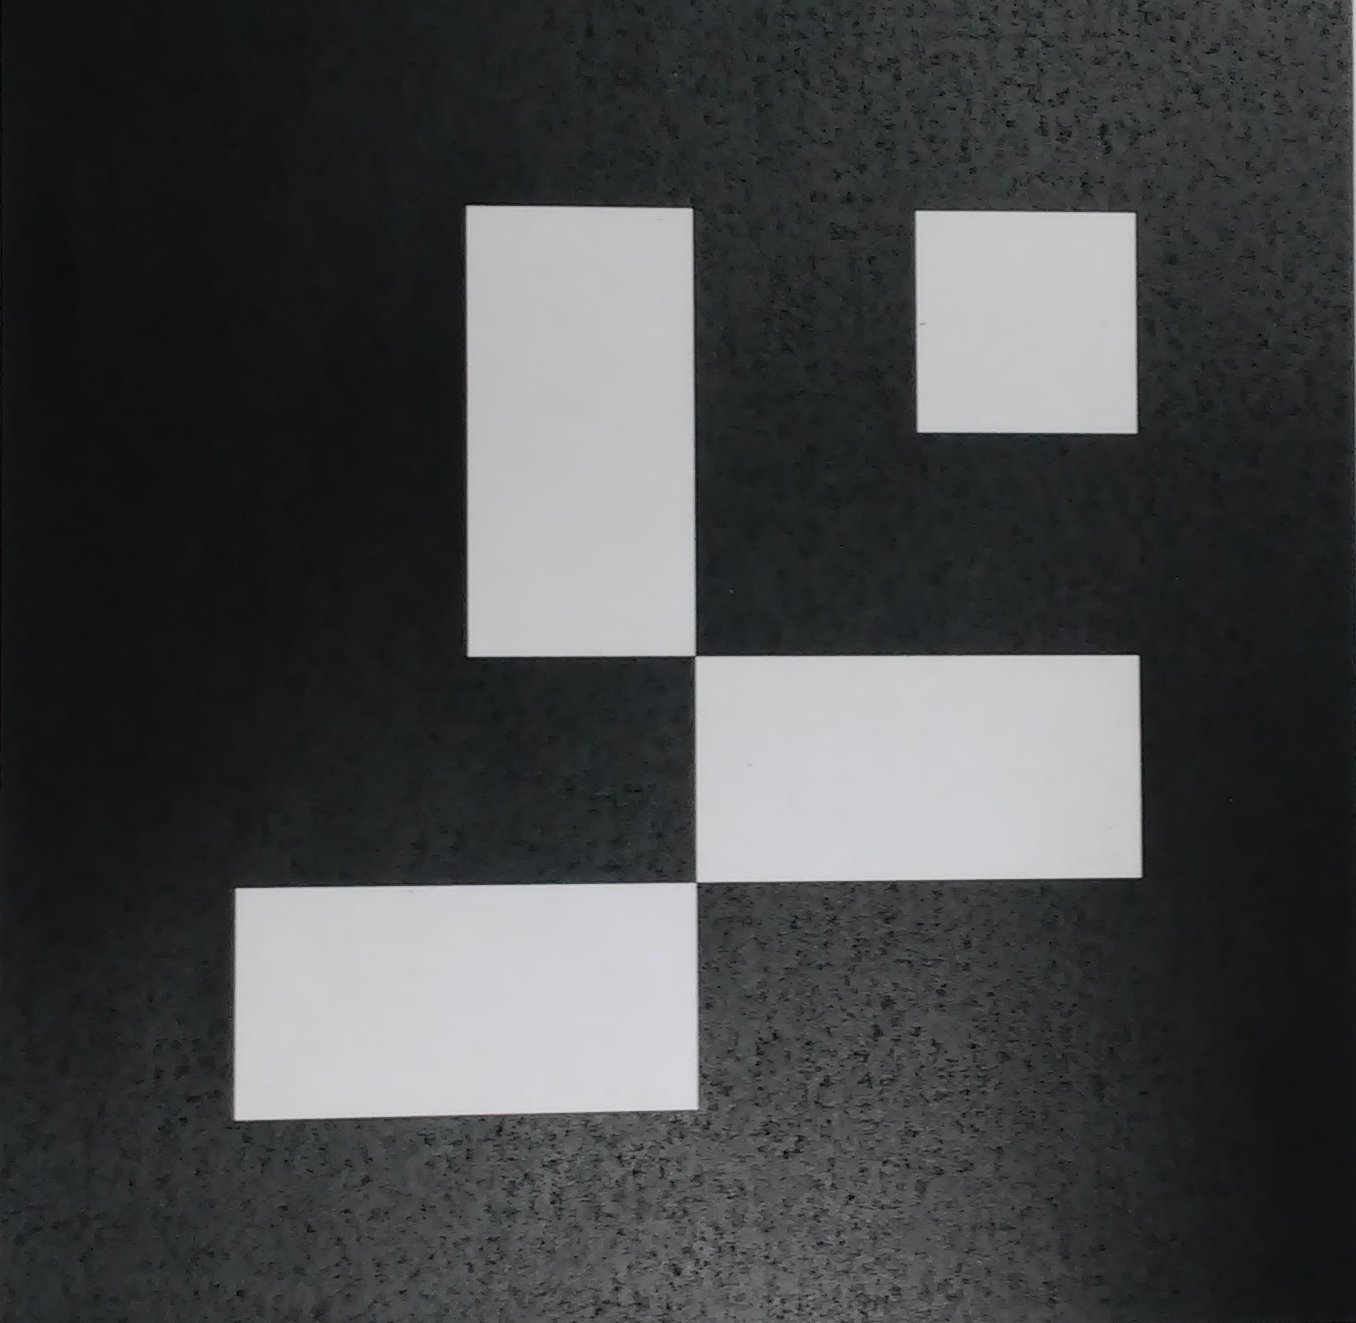
\includegraphics[width = 0.4\linewidth]{patch.jpg}
	\caption{Image of the patch used}
	\label{ref:patch}
\end{figure}

These patches have to be applied on top of the robot.
To be able to attach one of those patches to our robot, we needed to add some structure on top of the robot (see figure \ref{fig:robot}).

\begin{figure}[H]
    \centering
    \begin{subfigure}[b]{0.3\textwidth}
        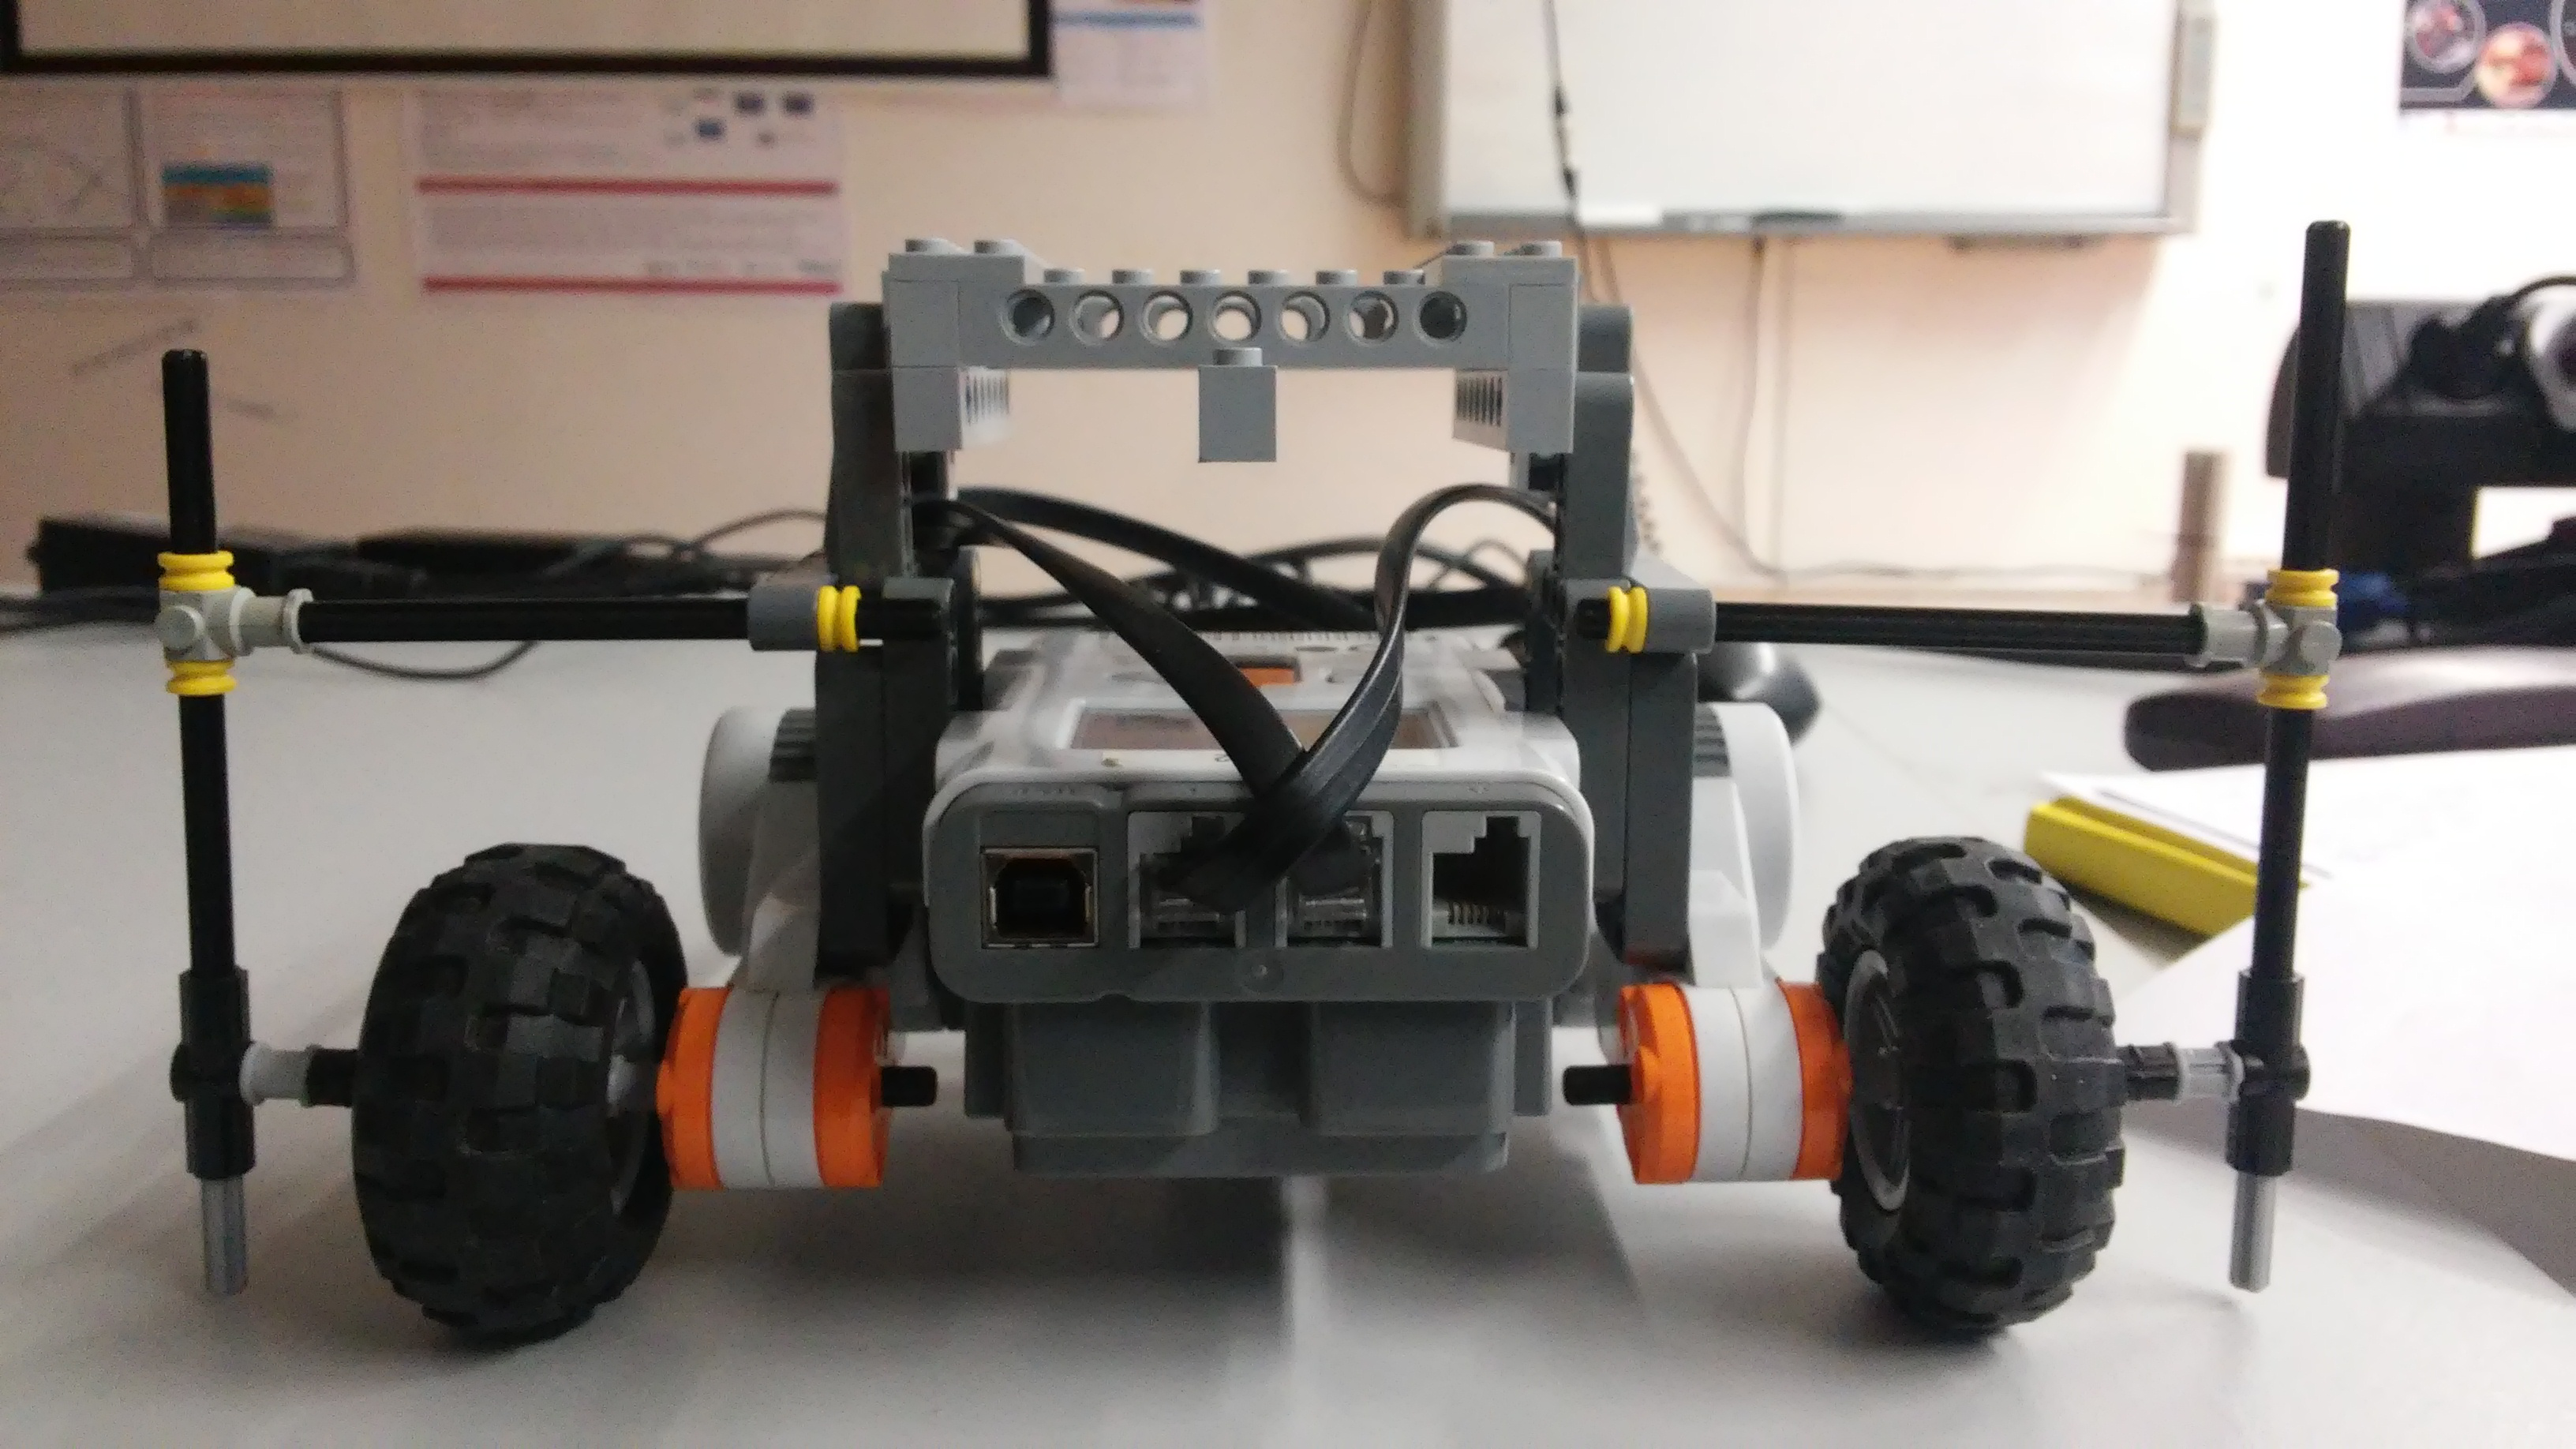
\includegraphics[width=\textwidth]{front.jpg}
        \caption{Front View}
        \label{fig:front}
    \end{subfigure}
    ~ %add desired spacing between images, e. g. ~, \quad, \qquad, \hfill etc. 
      %(or a blank line to force the subfigure onto a new line)
    \begin{subfigure}[b]{0.3\textwidth}
        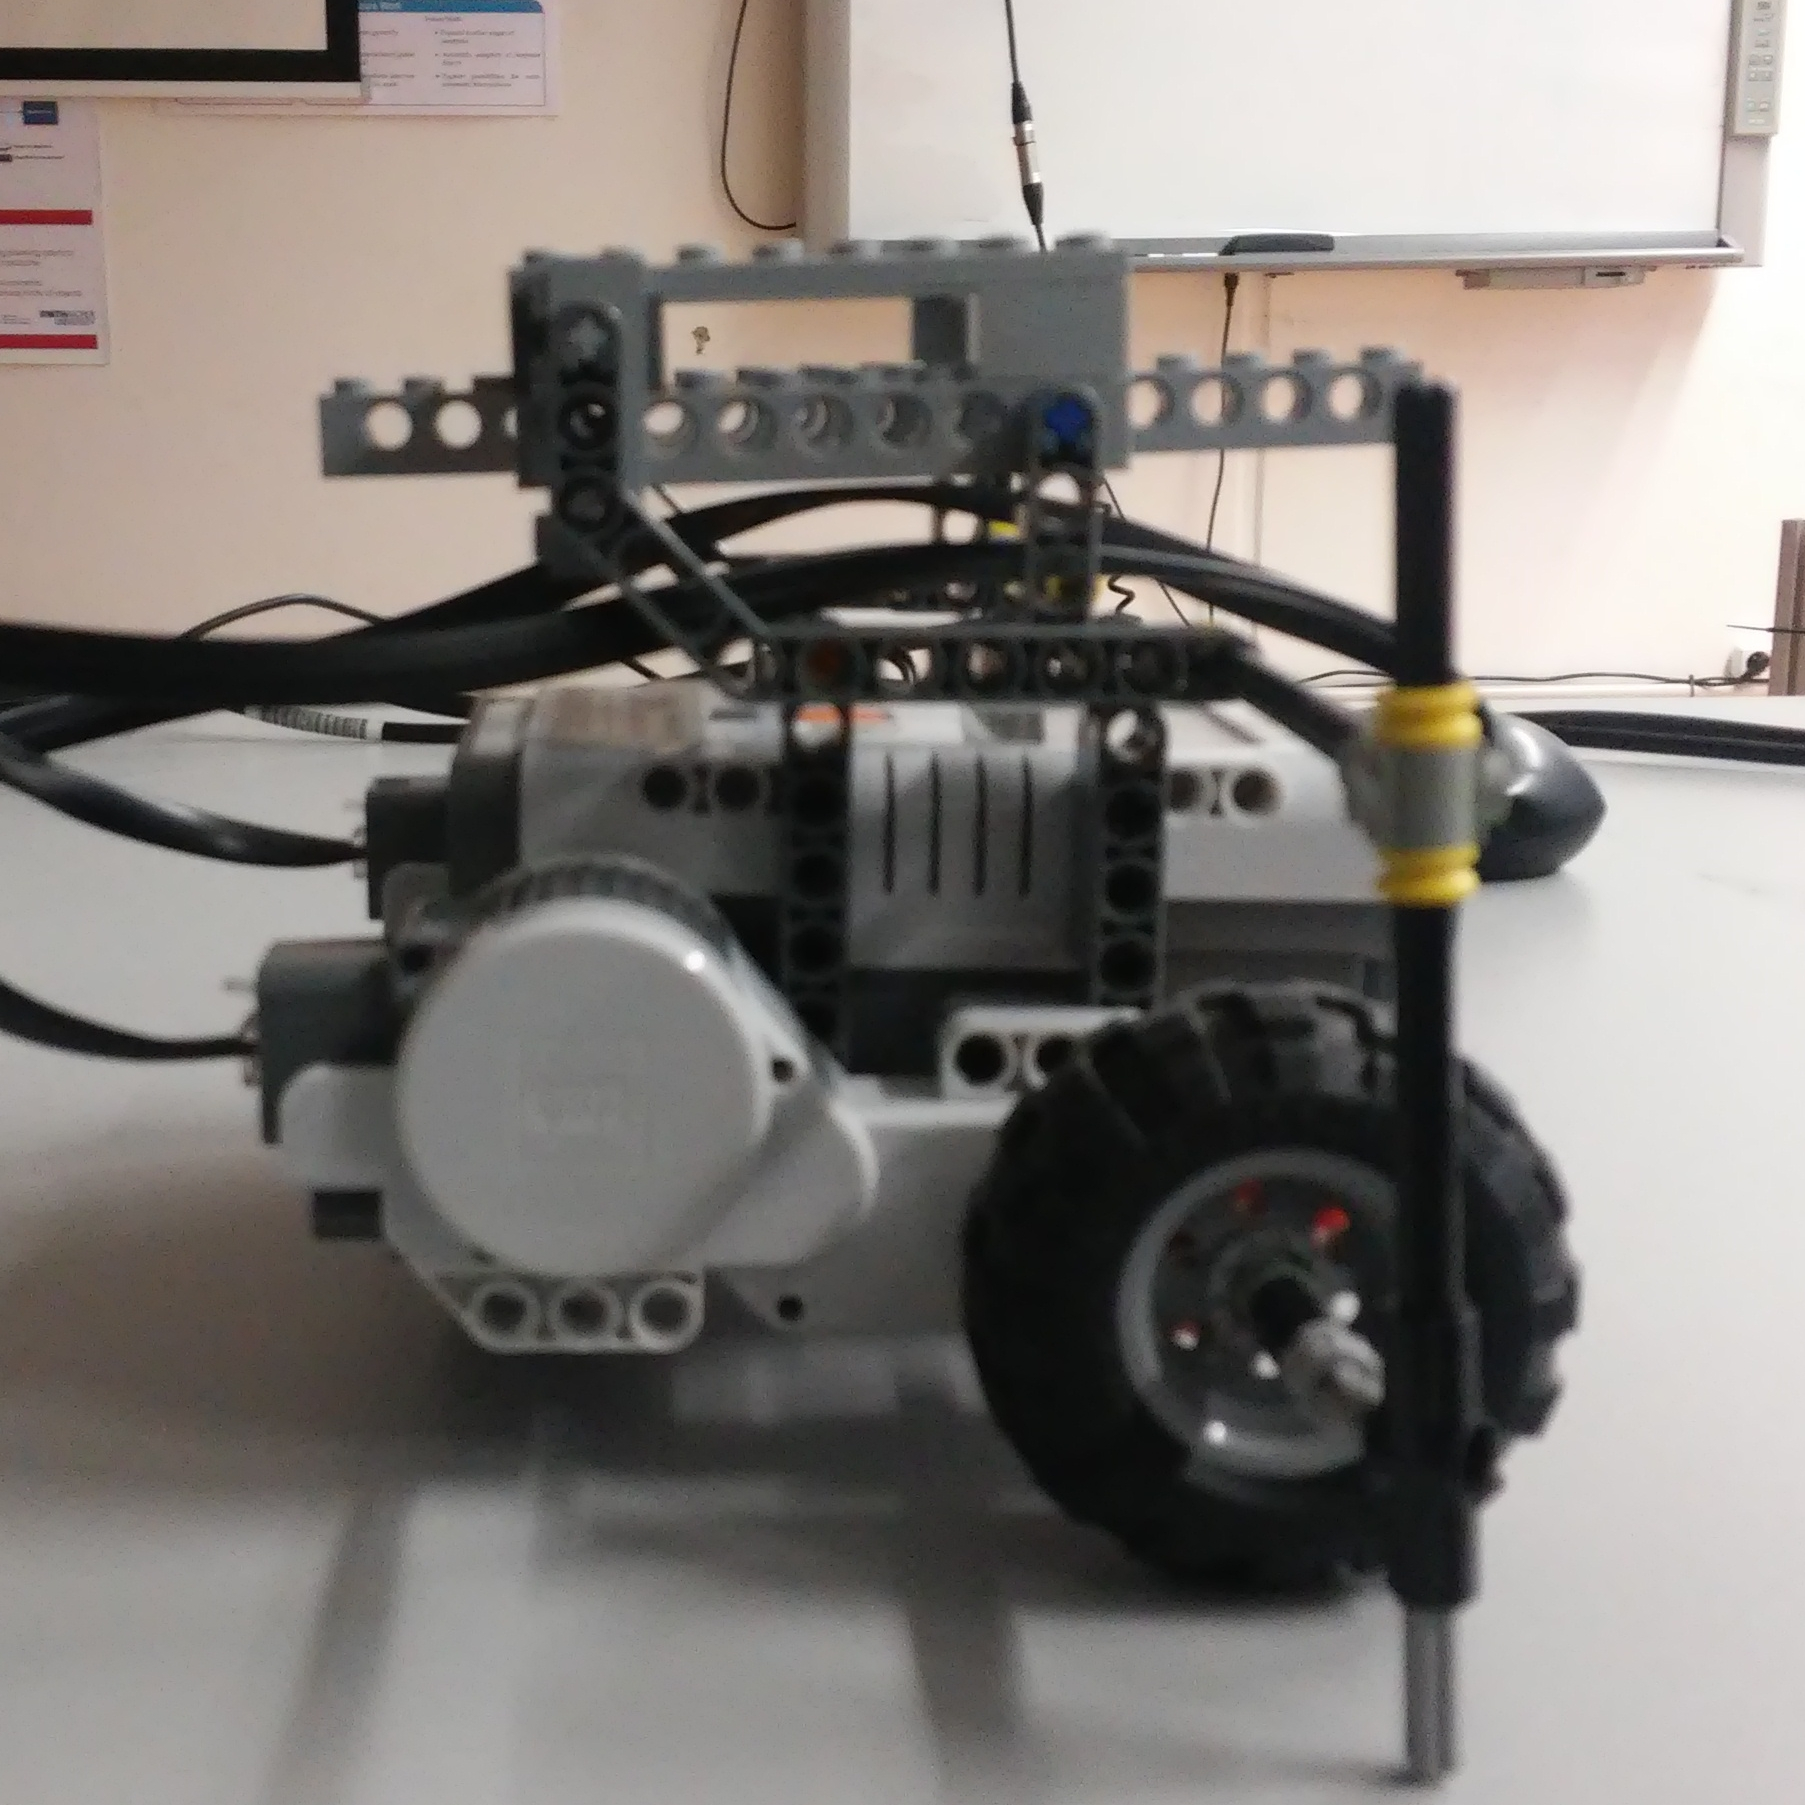
\includegraphics[width=\textwidth]{side.jpg}
        \caption{Side View}
        \label{fig:side}
    \end{subfigure}
    \begin{subfigure}[b]{0.3\textwidth}
        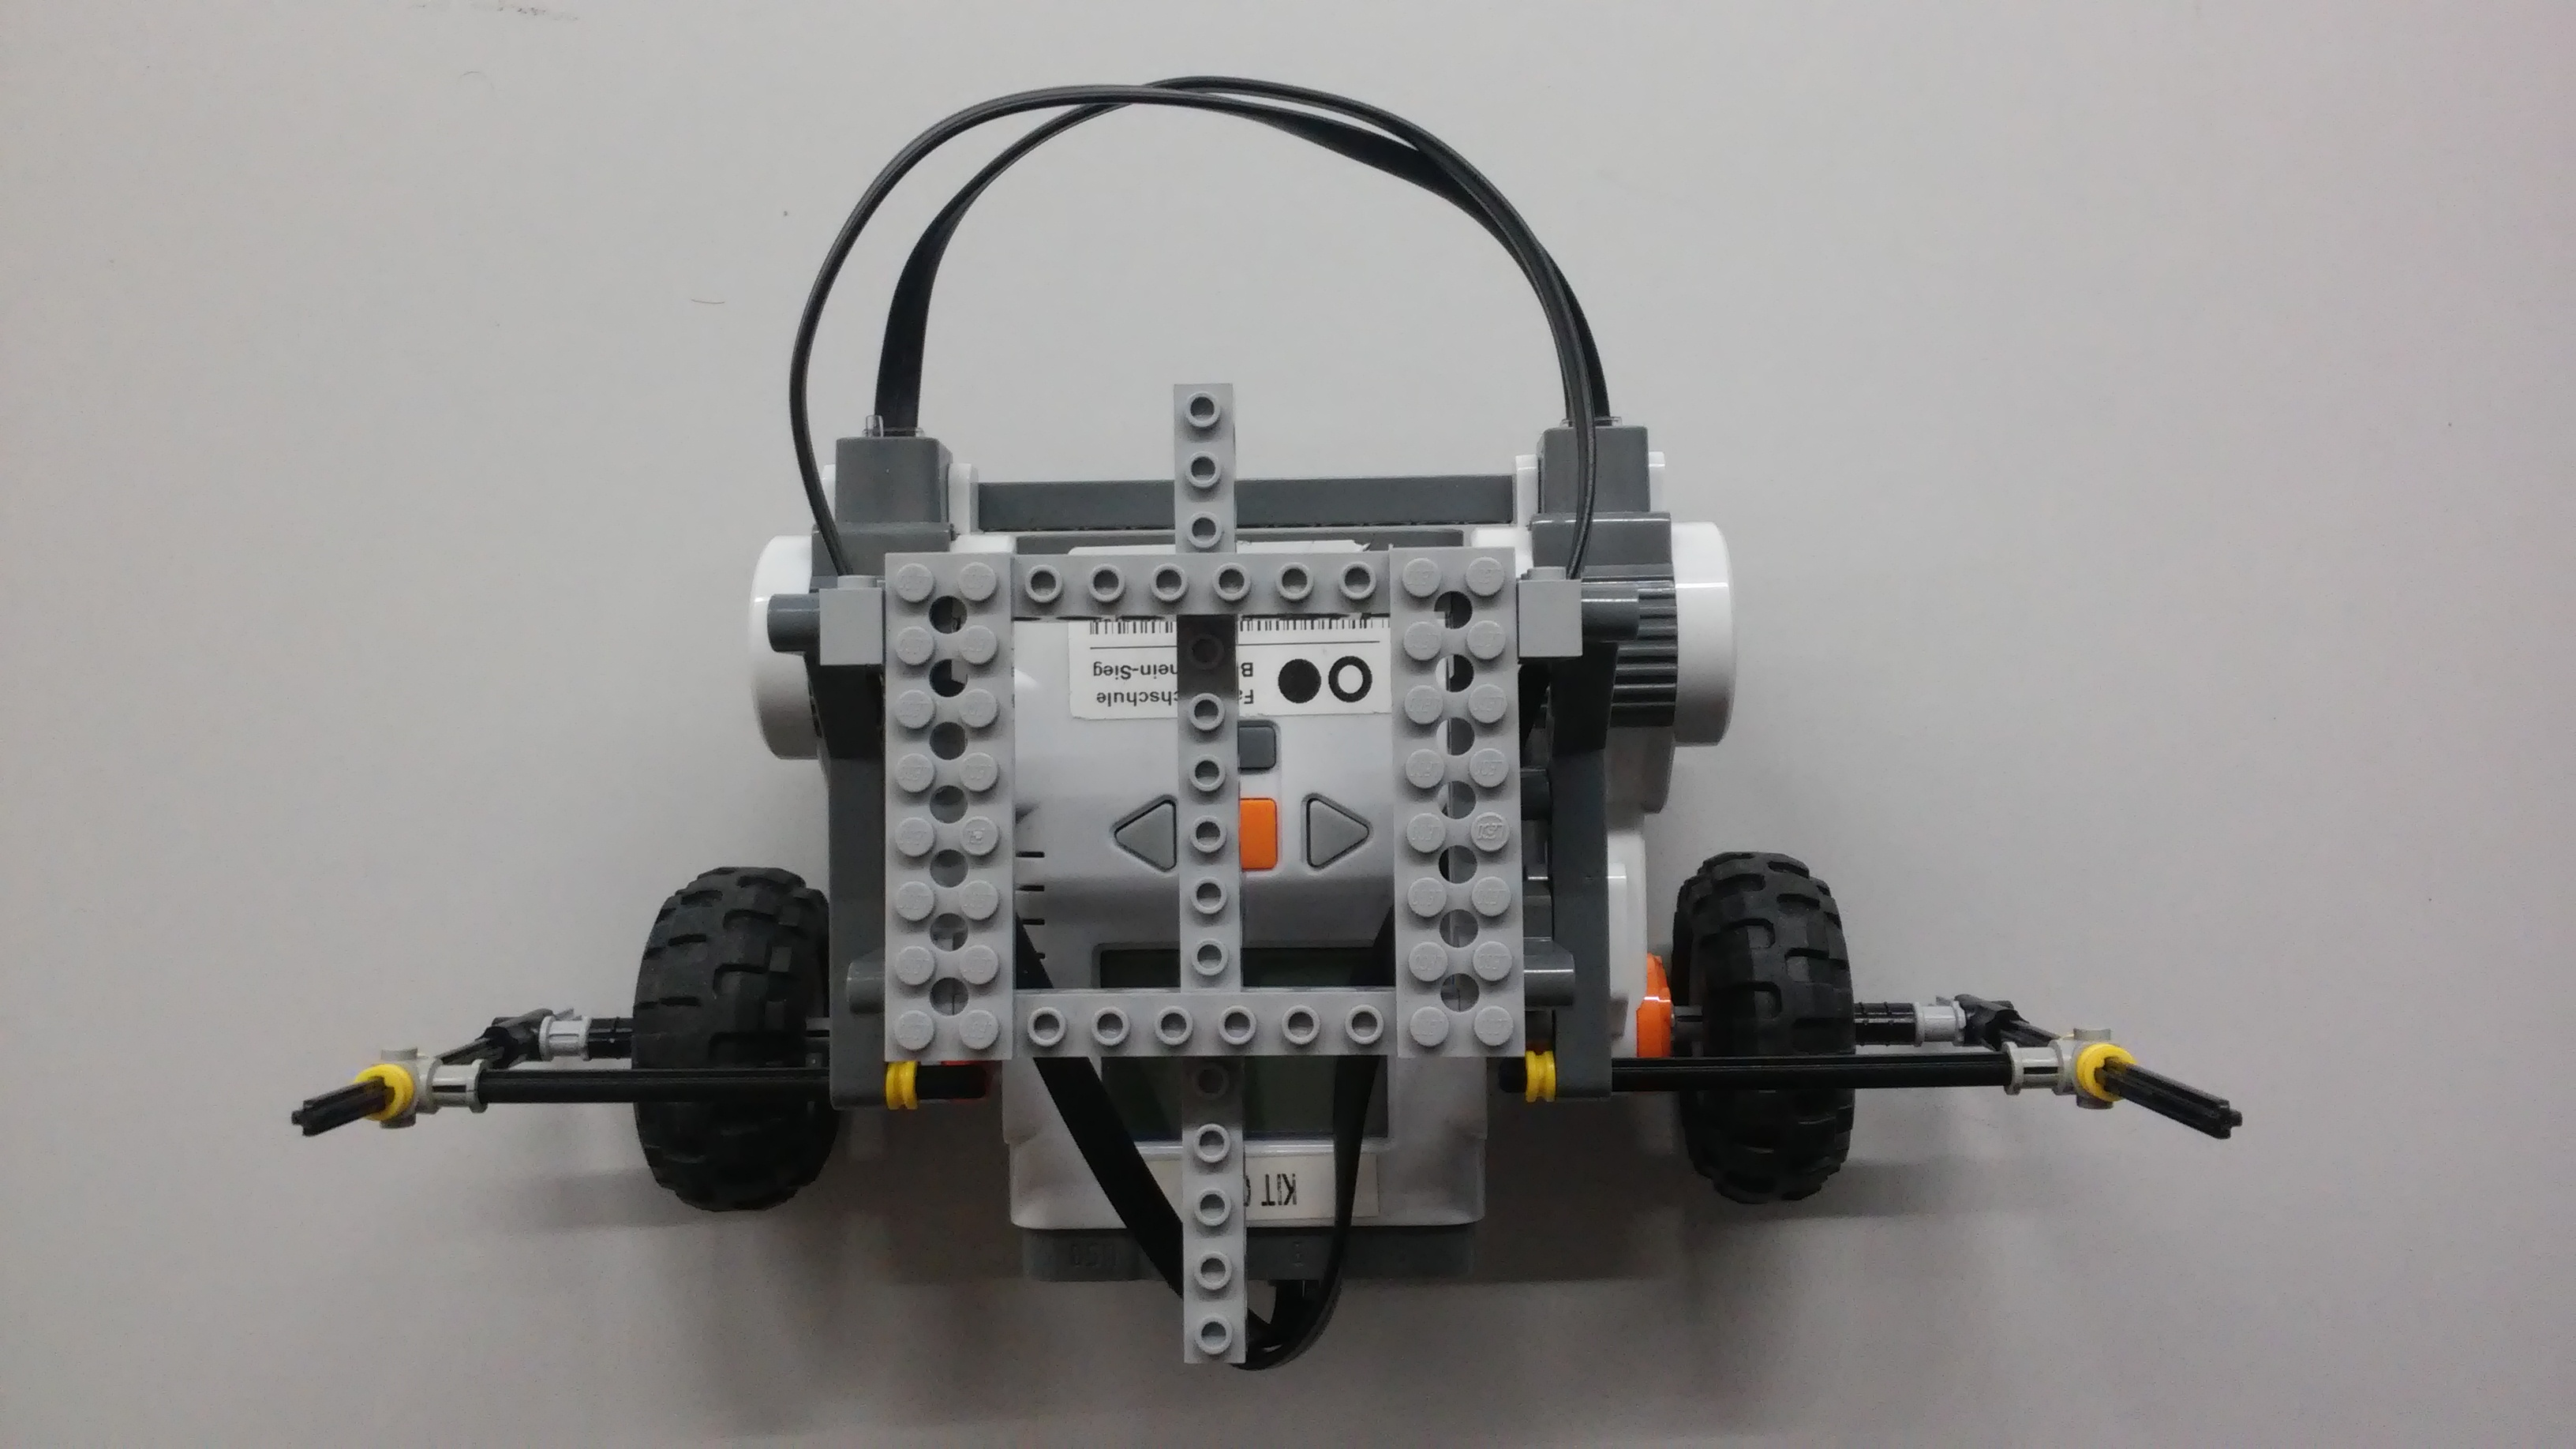
\includegraphics[width=\textwidth]{top.jpg}
        \caption{Top View}
        \label{fig:top}
    \end{subfigure}
    \caption{Improved Robot}\label{fig:robot}
\end{figure}

Using this structure we fixed the patch on top of the robot in a way that the center of the patch aligns with the center of motion of the robot.
The measured poses can be retrieved from a log file created in the measurement process.


\section{Tests}
The robot has been placed in the arena and the AICISS system recognized its position.
Its pose is been given by its by x and y position plus its orientation.
We tested two scenarios and compared resulting values with expectations.
\begin{itemize}
	\item Move robot by one meter in a straight line
	\item Turn the robot by 180 degrees
\end{itemize}
Our measurement probably include some errors that we introduced while measuring. 
We should do these kind of experiments repeatedly and use the average to have a valid estimation about the error.

\subsection{Straight Line}
Position start: [3316 2870]\\
Position end: [3325.5 3854.5]\\
Measured distance moved: 984.84mm\\
Expected distance moved: 1000.0mm

The measurement is about 1.5cm off.

\subsection{Orientation}
Orientation start: 3.08\\
Orientation end: 6.20\\
Expected Value: 6.22

The measurement is off by 0.02 radiant.

\begin{figure}[H]
    \centering
    \begin{subfigure}[b]{0.45\textwidth}
        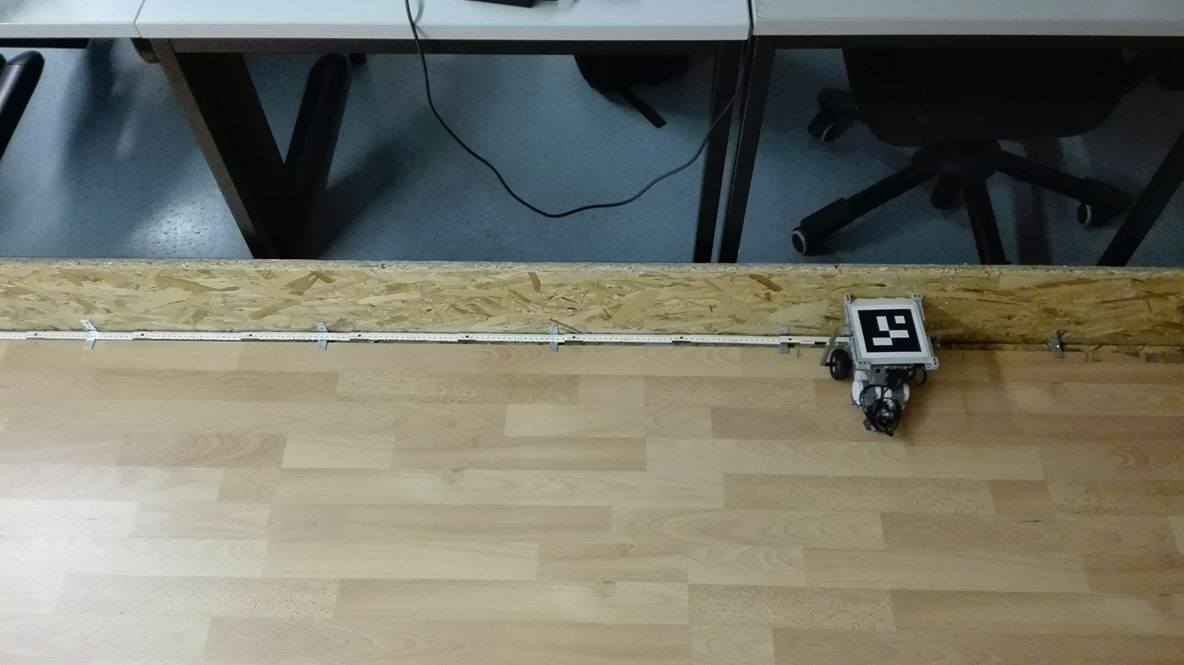
\includegraphics[width=\textwidth]{start.jpg}
        \caption{Start position of test}
        \label{fig:start}
    \end{subfigure}
    ~ %add desired spacing between images, e. g. ~, \quad, \qquad, \hfill etc. 
      %(or a blank line to force the subfigure onto a new line)
    \begin{subfigure}[b]{0.45\textwidth}
        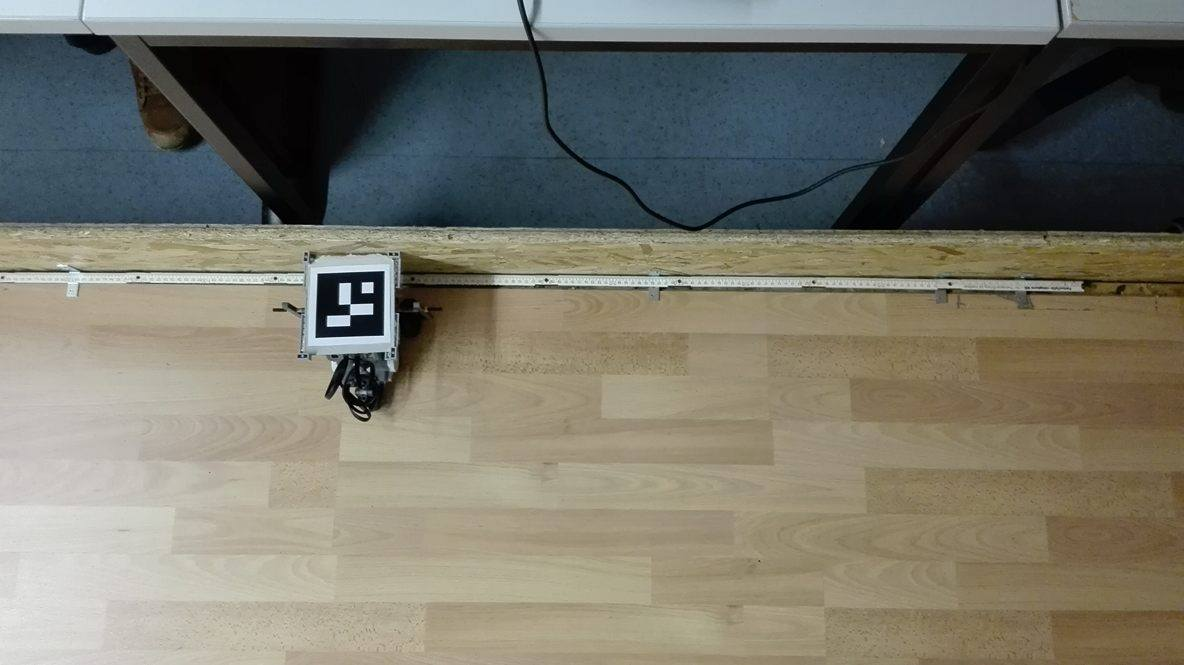
\includegraphics[width=\textwidth]{end.jpg}
        \caption{End position of test}
        \label{fig:end}
    \end{subfigure}
    \caption{Straight Line Movement Test}\label{fig:test}
\end{figure}



\bibliographystyle{plain}
\bibliography{bibtex.bib}






\end{document}